\newpage
\section{Polar de arrasto transônica}

Para levantar a polar transônica do perfil otimizado, o \texttt{single\_run}
foi adaptado para varrer o ângulo de ataque no intervalo
$\alpha_{\mathrm{proj}} \pm 2^\circ$ em passos de $0{,}5^\circ$, mantendo o
mesmo solver, malha e critérios de convergência da otimização, e coletando
$c_\ell$ e $c_d$ de cada simulação Euler. A mesma varredura foi aplicada ao
RAE~2822 --- perfil supercrítico clássico, cujos coeficientes CST acompanham
o \texttt{single\_run} --- como referência de comparação. A
Figura~\ref{fig:polar_transonica} sobrepõe as duas polares, com o ponto de
projeto destacado.

\begin{figure}[H]
    \centering
    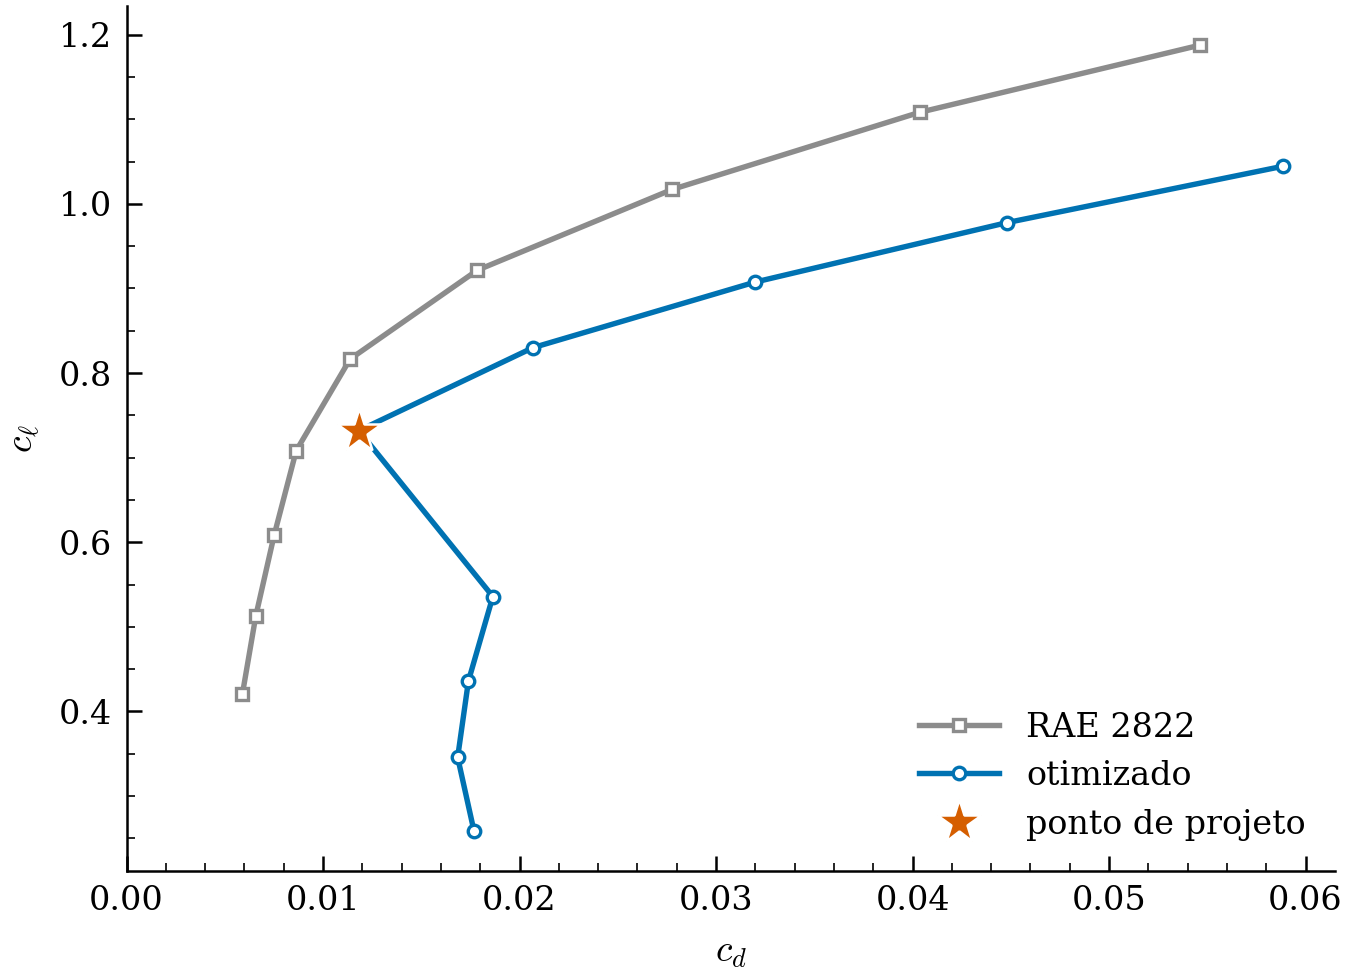
\includegraphics[width=0.8\textwidth]{images/06_polar/polar_transonica.png}
    \caption{Polar de arrasto transônica $c_\ell \times c_d$ do perfil
    otimizado com o ponto de projeto destacado, sobreposta à do RAE~2822
    ($M_n = 0{,}7196$).}\label{fig:polar_transonica}
\end{figure}

A peculiaridade da polar salta à vista: o perfil otimizado tem um
\emph{poço de arrasto} (``drag bucket'') estreito e profundo, centrado
exatamente no $c_\ell$ de projeto. Meio grau abaixo do ponto de projeto o
$c_d$ sobe $60\%$; meio grau acima, $76\%$. Uma varredura mais fina, com
passo de $0{,}1^\circ$, mostra que a degradação começa imediatamente:
$+0{,}2^\circ$ já custa $+26\%$ de arrasto.

Um resultado tão localizado exige verificação antes de ser aceito, e três
foram feitas. Primeiro, o resíduo de cada ponto da varredura foi
inspecionado: os pontos que estagnaram antes da tolerância foram reavaliados
com CFL reduzido até a convergência plena, e o $c_d$ mudou no máximo
$0{,}04\%$ --- a polar não é artefato de convergência. Segundo, o poço
sobrevive ao refinamento de malha: no nível 1,5 ele fica inclusive
\emph{mais} profundo (razão entre o maior e o menor $c_d$ na faixa de
$\pm0{,}4^\circ$ subindo de $1{,}60$ para $1{,}89$), com o mínimo
permanecendo no ponto de projeto --- o otimizador não explorou uma
peculiaridade da malha grossa. Terceiro, o próprio ótimo foi validado por
multistart e cortes unidimensionais (Seção~4).

O poço estreito é bom ou ruim para o projeto? É a assinatura esperada ---
e conhecida na literatura --- da otimização \emph{mono-ponto}: o otimizador
molda o teto supersônico da Figura~\ref{fig:mach_overlay} para uma condição
específica de $M$ e $c_\ell$, e qualquer desvio reconstrói o choque que ele
desmontou. No ponto de projeto, isso é excelente: é onde a aeronave passa a
maior parte da missão. Fora dele, é um risco real: variações de peso ao
longo do cruzeiro, rajadas, manobras e mudanças de altitude deslocam o
$c_\ell$ da seção, e a margem de \emph{buffet} fica estreita. Há ainda uma
dependência de projeto: o $c_\ell$ de cada estação foi derivado assumindo
distribuição de sustentação elíptica, que a torção da asa (próximo
laboratório) precisa confirmar --- se a distribuição real se desviar, o
perfil operará fora do fundo do poço. As duas respostas naturais, deixadas
como próximos passos, são a otimização \emph{multiponto} (minimizar uma
média ponderada de $c_d$ em 2--3 condições vizinhas, alargando o poço ao
custo de alguns \emph{counts} no ponto nominal) e a realimentação do
$c_\ell$ de projeto após o laboratório de torção.

Quanto à comparação com o RAE~2822, ela pede honestidade sobre espessura: o
RAE~2822 tem $t/c = 0{,}121$, enquanto o nosso perfil carrega
$t/c = 0{,}1772$ --- $46\%$ mais espessura, imposta pela restrição
estrutural da asa. Espessura custa arrasto de onda, e ainda assim o perfil
otimizado atinge, no seu ponto de projeto, um $c_d$ da mesma ordem do
RAE~2822 no mesmo $c_\ell$. A polar do RAE~2822 é visivelmente mais larga
--- vantagem de um perfil desenhado (e refinado ao longo de décadas) para
robustez fora de projeto, e não para um único ponto.
